\documentclass{standalone}
\usepackage{tikz}
\usetikzlibrary{patterns, positioning}
\usepackage[sfdefault]{ClearSans} %% option 'sfdefault' activates Clear Sans as the default text font
\usepackage[T1]{fontenc}

\begin{document}
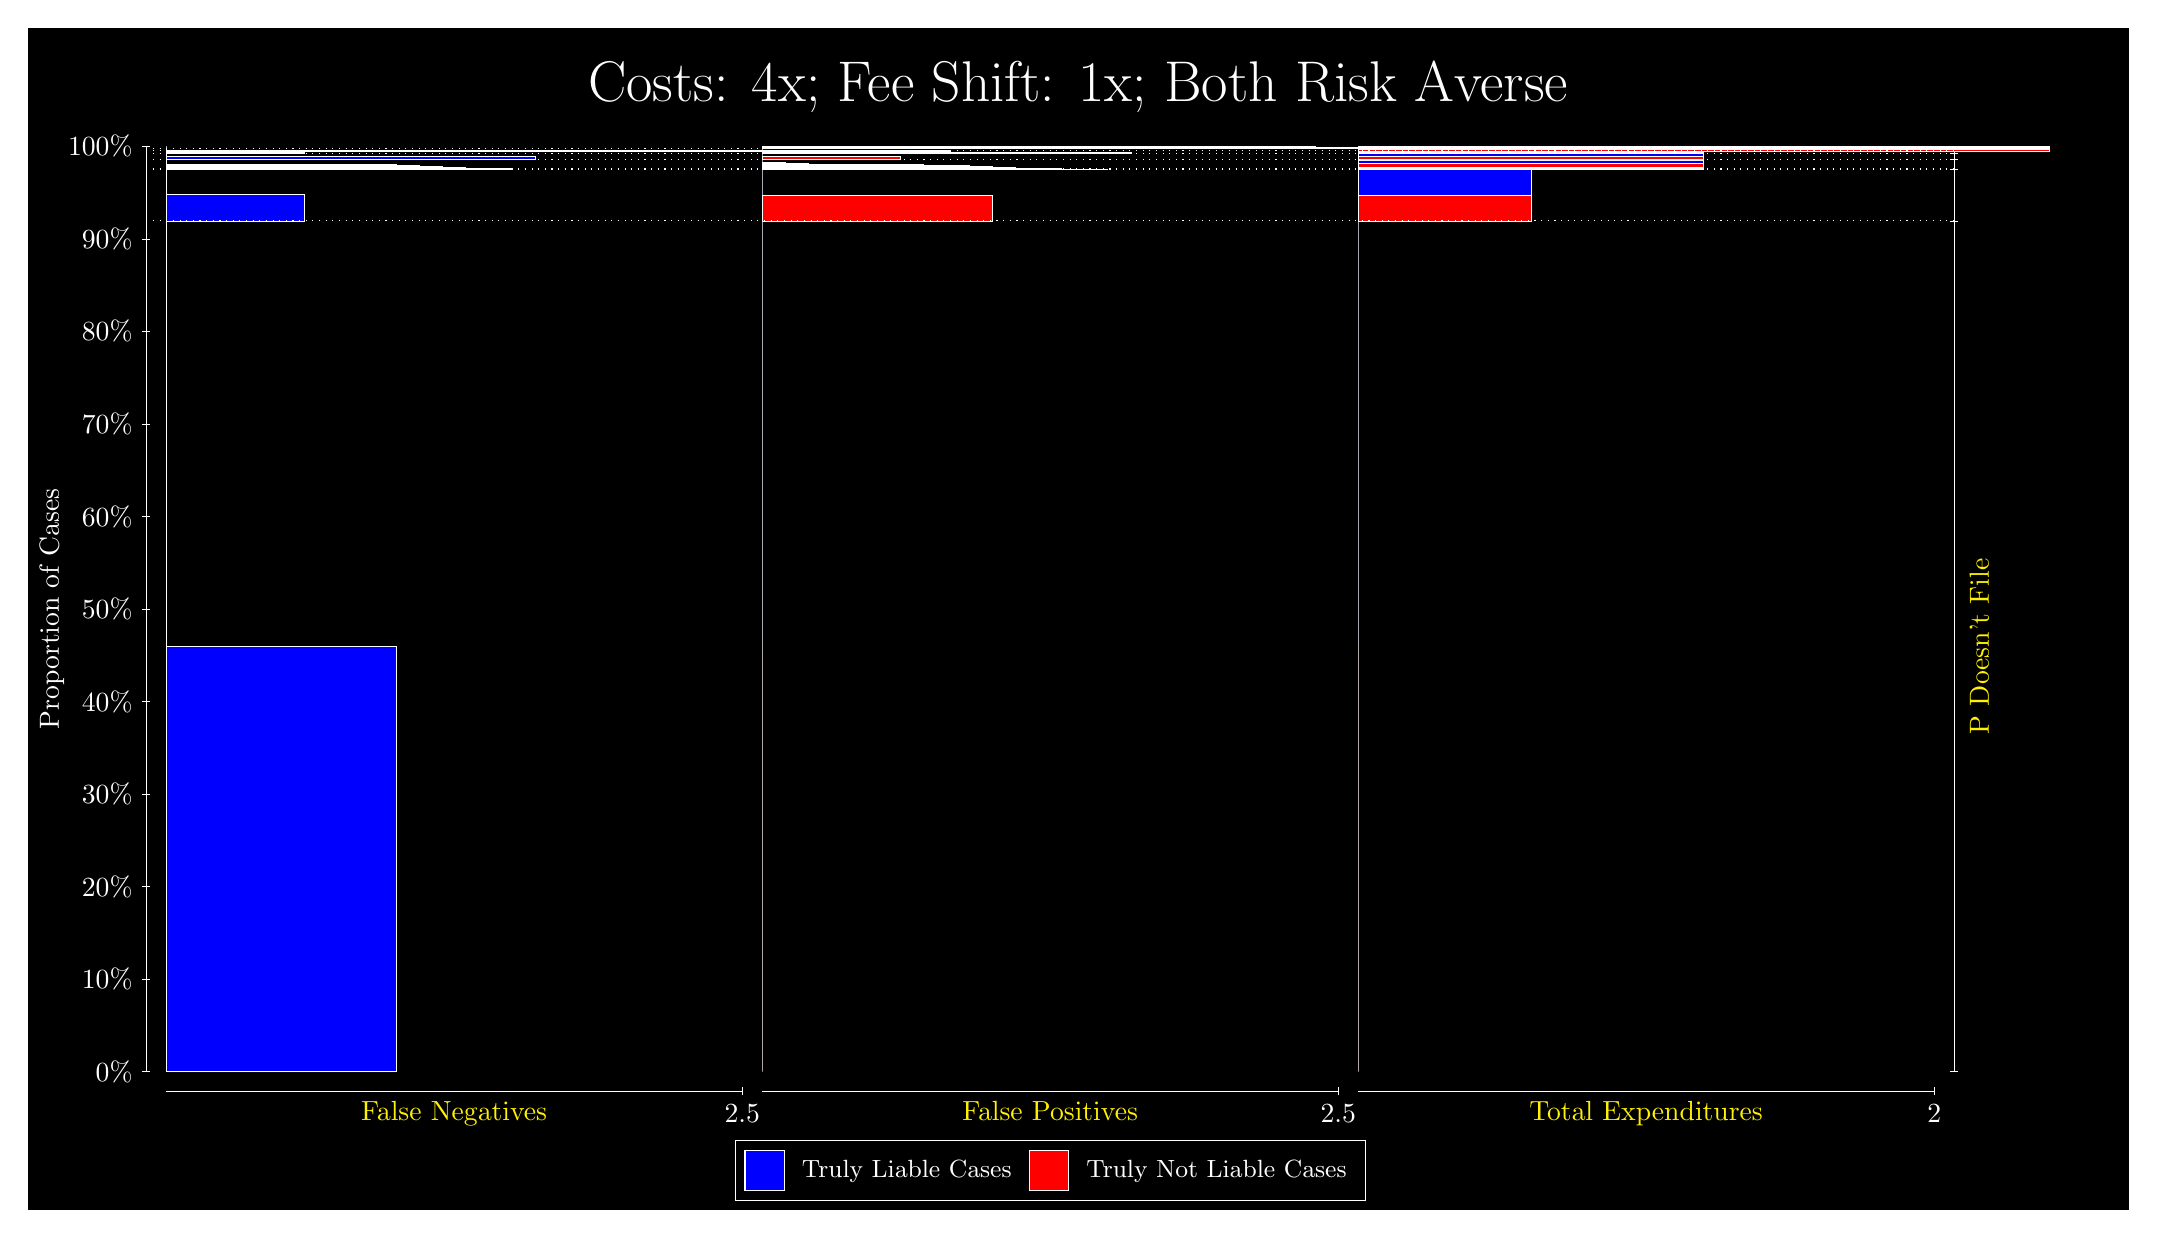
\begin{tikzpicture}
\draw[fill=black] (0,0) rectangle (26.667,15);
\draw[text=white] (0,13.5) rectangle (26.667,15) node[midway] {\huge Costs: 4x; Fee Shift: 1x; Both Risk Averse};
\draw[white, very thin] (1.5,1.75) -- (1.5,13.5);
\node[rotate=90, text=white, anchor=center] at (0.3, 7.625) {Proportion of Cases};
\draw[white, very thin] (1.45,1.75) -- (1.55,1.75);
\node[text=white, anchor=east] at (1.45, 1.75) {0\%};
\draw[white, very thin] (1.45,2.925) -- (1.55,2.925);
\node[text=white, anchor=east] at (1.45, 2.925) {10\%};
\draw[white, very thin] (1.45,4.1) -- (1.55,4.1);
\node[text=white, anchor=east] at (1.45, 4.1) {20\%};
\draw[white, very thin] (1.45,5.275) -- (1.55,5.275);
\node[text=white, anchor=east] at (1.45, 5.275) {30\%};
\draw[white, very thin] (1.45,6.45) -- (1.55,6.45);
\node[text=white, anchor=east] at (1.45, 6.45) {40\%};
\draw[white, very thin] (1.45,7.625) -- (1.55,7.625);
\node[text=white, anchor=east] at (1.45, 7.625) {50\%};
\draw[white, very thin] (1.45,8.8) -- (1.55,8.8);
\node[text=white, anchor=east] at (1.45, 8.8) {60\%};
\draw[white, very thin] (1.45,9.975) -- (1.55,9.975);
\node[text=white, anchor=east] at (1.45, 9.975) {70\%};
\draw[white, very thin] (1.45,11.15) -- (1.55,11.15);
\node[text=white, anchor=east] at (1.45, 11.15) {80\%};
\draw[white, very thin] (1.45,12.325) -- (1.55,12.325);
\node[text=white, anchor=east] at (1.45, 12.325) {90\%};
\draw[white, very thin] (1.45,13.5) -- (1.55,13.5);
\node[text=white, anchor=east] at (1.45, 13.5) {100\%};

\draw[white, very thin] (24.457,1.75) -- (24.457,13.5);
\draw[white, very thin] (24.407,1.75) -- (24.507,1.75);
\node[anchor=west] at (24.407, 1.75) {};
\draw[white, very thin] (24.407,12.553) -- (24.507,12.553);
\node[anchor=west] at (24.407, 12.553) {};
\draw[white, very thin] (24.407,13.212) -- (24.507,13.212);
\node[anchor=west] at (24.407, 13.212) {};
\draw[white, very thin] (24.407,13.334) -- (24.507,13.334);
\node[anchor=west] at (24.407, 13.334) {};
\draw[white, very thin] (24.407,13.409) -- (24.507,13.409);
\node[anchor=west] at (24.407, 13.409) {};
\draw[white, very thin] (24.407,13.443) -- (24.507,13.443);
\node[anchor=west] at (24.407, 13.443) {};
\draw[white, very thin] (24.407,13.477) -- (24.507,13.477);
\node[anchor=west] at (24.407, 13.477) {};
\draw[white, very thin] (24.407,13.5) -- (24.507,13.5);
\node[anchor=west] at (24.407, 13.5) {};

\draw[white, very thin, fill=blue] (1.75,1.75) rectangle (4.6775,7.1515);
\draw[white, very thin, fill=red] (1.75,7.1515) rectangle (1.75,12.553);
\draw[white, very thin, fill=blue] (1.75,12.553) rectangle (3.5065,12.885);
\draw[white, very thin, fill=red] (1.75,12.885) rectangle (1.75,13.212);
\draw[white, very thin, fill=blue] (1.75,13.212) rectangle (6.1413,13.222);
\draw[white, very thin, fill=blue] (1.75,13.222) rectangle (5.8486,13.226);
\draw[white, very thin, fill=blue] (1.75,13.226) rectangle (5.5558,13.24);
\draw[white, very thin, fill=blue] (1.75,13.24) rectangle (5.2631,13.252);
\draw[white, very thin, fill=blue] (1.75,13.252) rectangle (4.9703,13.265);
\draw[white, very thin, fill=blue] (1.75,13.265) rectangle (4.6775,13.268);
\draw[white, very thin, fill=blue] (1.75,13.268) rectangle (4.3848,13.271);
\draw[white, very thin, fill=blue] (1.75,13.271) rectangle (4.092,13.272);
\draw[white, very thin, fill=blue] (1.75,13.272) rectangle (3.7993,13.274);
\draw[white, very thin, fill=red] (1.75,13.274) rectangle (1.75,13.334);
\draw[white, very thin, fill=blue] (1.75,13.334) rectangle (6.4341,13.37);
\draw[white, very thin, fill=red] (1.75,13.37) rectangle (1.75,13.409);
\draw[white, very thin, fill=blue] (1.75,13.409) rectangle (3.5065,13.427);
\draw[white, very thin, fill=red] (1.75,13.427) rectangle (1.75,13.443);
\draw[white, very thin, fill=blue] (1.75,13.443) rectangle (11.704,13.455);
\draw[white, very thin, fill=red] (1.75,13.455) rectangle (1.75,13.477);
\draw[white, very thin, fill=red] (1.75,13.477) rectangle (1.75,13.486);
\draw[white, very thin, fill=blue] (1.75,13.486) rectangle (1.75,13.5);
\draw[white, very thin, fill=red] (9.3189,1.75) rectangle (9.3189,7.1515);
\draw[white, very thin, fill=blue] (9.3189,7.1515) rectangle (9.3189,12.553);
\draw[white, very thin, fill=red] (9.3189,12.553) rectangle (12.246,12.88);
\draw[white, very thin, fill=blue] (9.3189,12.88) rectangle (9.3189,13.212);
\draw[white, very thin, fill=red] (9.3189,13.212) rectangle (13.71,13.213);
\draw[white, very thin, fill=red] (9.3189,13.213) rectangle (13.417,13.214);
\draw[white, very thin, fill=red] (9.3189,13.214) rectangle (13.125,13.217);
\draw[white, very thin, fill=red] (9.3189,13.217) rectangle (12.832,13.22);
\draw[white, very thin, fill=red] (9.3189,13.22) rectangle (12.539,13.232);
\draw[white, very thin, fill=red] (9.3189,13.232) rectangle (12.246,13.242);
\draw[white, very thin, fill=red] (9.3189,13.242) rectangle (11.954,13.255);
\draw[white, very thin, fill=red] (9.3189,13.255) rectangle (11.661,13.259);
\draw[white, very thin, fill=red] (9.3189,13.259) rectangle (11.368,13.272);
\draw[white, very thin, fill=blue] (9.3189,13.272) rectangle (10.783,13.273);
\draw[white, very thin, fill=blue] (9.3189,13.273) rectangle (10.49,13.275);
\draw[white, very thin, fill=blue] (9.3189,13.275) rectangle (10.197,13.278);
\draw[white, very thin, fill=blue] (9.3189,13.278) rectangle (9.9044,13.281);
\draw[white, very thin, fill=blue] (9.3189,13.281) rectangle (9.6116,13.294);
\draw[white, very thin, fill=blue] (9.3189,13.294) rectangle (9.3189,13.334);
\draw[white, very thin, fill=red] (9.3189,13.334) rectangle (11.075,13.374);
\draw[white, very thin, fill=blue] (9.3189,13.374) rectangle (9.3189,13.409);
\draw[white, very thin, fill=red] (9.3189,13.409) rectangle (14.003,13.425);
\draw[white, very thin, fill=blue] (9.3189,13.425) rectangle (11.075,13.443);
\draw[white, very thin, fill=red] (9.3189,13.443) rectangle (9.3189,13.464);
\draw[white, very thin, fill=blue] (9.3189,13.464) rectangle (9.3189,13.477);
\draw[white, very thin, fill=red] (9.3189,13.477) rectangle (19.273,13.486);
\draw[white, very thin, fill=blue] (9.3189,13.486) rectangle (16.345,13.5);
\draw[white, very thin, fill=red] (16.888,1.75) rectangle (16.888,7.1515);
\draw[white, very thin, fill=blue] (16.888,7.1515) rectangle (16.888,12.553);
\draw[white, very thin, fill=red] (16.888,12.553) rectangle (19.083,12.88);
\draw[white, very thin, fill=blue] (16.888,12.88) rectangle (19.083,13.212);
\draw[white, very thin, fill=red] (16.888,13.212) rectangle (21.279,13.223);
\draw[white, very thin, fill=blue] (16.888,13.223) rectangle (21.279,13.235);
\draw[white, very thin, fill=red] (16.888,13.235) rectangle (21.279,13.28);
\draw[white, very thin, fill=blue] (16.888,13.28) rectangle (21.279,13.326);
\draw[white, very thin, fill=red] (16.888,13.326) rectangle (21.279,13.33);
\draw[white, very thin, fill=blue] (16.888,13.33) rectangle (21.279,13.334);
\draw[white, very thin, fill=red] (16.888,13.334) rectangle (21.279,13.374);
\draw[white, very thin, fill=blue] (16.888,13.374) rectangle (21.279,13.409);
\draw[white, very thin, fill=red] (16.888,13.409) rectangle (21.279,13.425);
\draw[white, very thin, fill=blue] (16.888,13.425) rectangle (21.279,13.443);
\draw[white, very thin, fill=red] (16.888,13.443) rectangle (25.67,13.464);
\draw[white, very thin, fill=blue] (16.888,13.464) rectangle (25.67,13.477);
\draw[white, very thin, fill=red] (16.888,13.477) rectangle (25.67,13.486);
\draw[white, very thin, fill=blue] (16.888,13.486) rectangle (25.67,13.5);
\draw[white, dotted] (1.5,12.553) -- (24.457,12.553);
\draw[white, dotted] (1.5,13.212) -- (24.457,13.212);
\draw[white, dotted] (1.5,13.334) -- (24.457,13.334);
\draw[white, dotted] (1.5,13.409) -- (24.457,13.409);
\draw[white, dotted] (1.5,13.443) -- (24.457,13.443);
\draw[white, dotted] (1.5,13.477) -- (24.457,13.477);
\draw[white, very thin] (1.75,1.5) -- (9.0689,1.5);
\node[text=yellow, anchor=north] at (5.4094, 1.5) {False Negatives};
\draw[white, very thin] (9.0689,1.45) -- (9.0689,1.55);
\node[text=white, anchor=north] at (9.0689, 1.45) {2.5};

\draw[white, very thin] (9.3189,1.5) -- (16.638,1.5);
\node[text=yellow, anchor=north] at (12.978, 1.5) {False Positives};
\draw[white, very thin] (16.638,1.45) -- (16.638,1.55);
\node[text=white, anchor=north] at (16.638, 1.45) {2.5};

\draw[white, very thin] (16.888,1.5) -- (24.207,1.5);
\node[text=yellow, anchor=north] at (20.547, 1.5) {Total Expenditures};
\draw[white, very thin] (24.207,1.45) -- (24.207,1.55);
\node[text=white, anchor=north] at (24.207, 1.45) {2};

\node[text=yellow, centered, rotate=90] at (24.777, 7.1515) {P Doesn't File};







\draw (12.978300999999998,1.5) node[draw=none] (baseCoordinate) {};
\begin{scope}[align=center]
        \matrix[scale=0.5, draw=white, below=0.5cm of baseCoordinate, nodes={draw}, column sep=0.1cm]{
            \node[rectangle, draw, minimum width=0.5cm, minimum height=0.5cm, fill=blue] {}; &
            \node[draw=none, font=\small, text=white] (B) {Truly Liable Cases}; &
            \node[rectangle, draw, minimum width=0.5cm, minimum height=0.5cm, fill=red] {}; &
            \node[draw=none, font=\small, text=white] (B) {Truly Not Liable Cases}; \\
            };
\end{scope}

\end{tikzpicture}
\end{document}